%%%%%%%%%%%%%%%%%%%% author.tex %%%%%%%%%%%%%%%%%%%%%%%%%%%%%%%%%%%
%
% sample root file for your "contribution" to a proceedings volume
%
% Use this file as a template for your own input.
%
%%%%%%%%%%%%%%%% Springer %%%%%%%%%%%%%%%%%%%%%%%%%%%%%%%%%%


\documentclass[runningheads]{llncs}%
% RECOMMENDED %%%%%%%%%%%%%%%%%%%%%%%%%%%%%%%%%%%%%%%%%%%%%%%%%%%
%
%%%%%%%%%%%%PACKAGES
\usepackage{url}
\def\UrlFont{\rmfamily}
%NEW
%Packages
%\usepackage{graphicx}
\usepackage{comment}
\usepackage{pagecolor,lipsum}% http://ctan.org/pkg/{pagecolor,lipsum}
% Use the postscript times font!
%\usepackage{times}
\usepackage{soul}
\usepackage{url}
\usepackage[hidelinks]{hyperref}
\usepackage[utf8]{inputenc}
\usepackage[small]{caption}
\usepackage{graphicx}
\usepackage{amsmath}
\usepackage{amsthm}
\usepackage{amssymb}
\usepackage{booktabs}
\usepackage{algorithm}
\usepackage{algorithmic}
\usepackage{comment}
\usepackage{subcaption}
\usepackage{multirow}
\usepackage{breakcites}
\usepackage{tabularx}
\usepackage[usenames,dvipsnames]{xcolor}
\usepackage{subcaption}
\usepackage[demo,abs]{overpic}
\usepackage[export]{adjustbox}
\usepackage[symbol]{footmisc}

%COMMANDS
\definecolor{red}{rgb}{0, 0, 0} 


\begin{document}
%\mainmatter              % start of a contribution

%\pagecolor{gray}

\title{Human-Swarm Teaming with Proximal Interactions}
%\thanks{This project was supported by the AXA Research Fund and the Alan Turing Institute funded project on Flexible Autonomy for Swarm Robotics. The authors would like to thank Guillermo Romero Moreno for his pointers to reducing computational complexity.}}
%
\titlerunning{Human-Swarm Teaming with Proximal Interactions}  % abbreviated title (for running head)
%                                     also used for the TOC unless
%                                     \toctitle is used
%
\author{Mohammad Divband Soorati\inst{1}\orcidID{0000-0001-6954-1284} \and \\
Dimitar Georgiev\inst{1}\orcidID{0000-0001-6114-5500} \and
Javad Ghofrani\inst{2}\orcidID{0000-0002-9249-7434} \and
Danesh Tarapore\inst{1}\orcidID{0000-0002-3226-6861} \and \\
Sarvapali Ramchurn\inst{1}\orcidID{0000-0001-9686-4302}}
%
\authorrunning{M. Divband Soorati et al.} % abbreviated author list (for running head)
%
% %%%% list of authors for the TOC (use if author list has to be modified)
% \tocauthor{Mohammad {Divband Soorati}, 
% Dimitar Georgiev, 
% Javad Ghofrani, 
% Danesh Tarapore, and 
% Sarvapali Ramchurn}

% 	\institute{Department of Computer Science, School of Engineering and Applied Science, Princeton University, Princeton, NJ, USA \and
% 		Springer Heidelberg, Heidelberg, Germany
% 		\email{lncs@springer.com}\\ \and
% 		ABC Institute, Rupert-Karls-University Heidelberg, Heidelberg, Germany\\
% 		\email{\{abc,lncs\}@uni-heidelberg.de}}
% 	% Author affiliation information should include the following, using the 
% 	% \institute{} and \email{} fields: department, faculty, university, 
% 	% company (if applicable), city, country, and email address. Do not include 
% 	% the street address or ZIP code (ANTS 2020 does not use a postal address).
% 	% The email address of the corresponding author is mandatory to include in
% 	% the \institute{} and \email{} fields.
% 	%
% 	\index{Author, First}
% 	\index{Author, Second}
% 	\index{Author, Third}

%
\institute{School of Electronics and Computer Science, University of Southampton, UK \\
\email{\{m.divband-soorati,dg1g17,d.s.tarapore,sdr1\}@soton.ac.uk}\\
%\url{http://www.springer.com/gp/computer-science/lncs} 
\and
Department of Informatics and Mathematics, Dresden University of Applied Sciences, Germany 
\email{javad.ghofrani@gmail.com}}

\maketitle              % typeset the title of the contribution

\begin{abstract}
%Autonomous swarms are capable of accomplishing simple tasks but when it comes to critical situations (e.g., disaster management) they cannot manage the whole mission. By establishing a human-swarm interaction we create a system that can outperform humans or autonomous swarms when working independently. We propose a human-swarm teaming with proximal interactions between human operators and robots in a multi-agent system. 
  One of the major challenges in a human-swarm interaction is acquiring global information about the swarm's state and visualizing it to the human operators. Continuous swarm observation requires global communication between the human operator and the swarm that limits scalability and comes with a high communication cost. In our approach, we only allow one-to-one communications in local neighborhoods between agent-agent and operator-agent. By doing so, we decrease the cognitive complexity of human-swarm interaction to $O(1)$. 
%We decrease the cognitive complexity of human-swarm interaction to $O(1)$ and allow the human agents to locally interact with the swarm. 
Agents collectively explore and map the environment by disseminating their observations and incorporating their neighboring agents' maps. Human operators then use these maps to estimate the swarm's state, manipulate the maps to control the swarm, and as a result, determine the level of autonomy of the swarm. We verify our approach with a disaster management scenario where a simulated aerial swarm is spread across a mission zone to explore an environment. 
  %The agents then collectively form a path to guide the human operators (e.g., firefighters) to the areas of interest. 
Our proposed method for human-swarm teaming with proximal interactions successfully guides a swarm to explore a mission area in a dynamic environment and allows a single operator to control the swarm. 
\keywords{Human-swarm interaction, Aerial swarms, Disaster management, Situation awareness}
\end{abstract}
%
\section{Introduction}
%Colors:\\
%\textcolor{red}{Green: Suggestions}\\
%\textcolor{brown}{Brown: includes some copied text from literature}\\
%{Black: our text}\\

%\textcolor{red}{why Swarm robotics?}\\
%- we don't want to use a single drone
Unmanned aerial vehicles are commonly used for acquiring information from remote areas with hazard situations. Many studies focused on developing methods for disaster management using a swarm of flying drones~\cite{innocente2019self, gkotsis2019swarm, busnel2019self}. Autonomous coordination between agents with the limited on-board computation and communication capacities of simple agents is a complex task~\cite{chung2018survey}. While flying swarms have promising future applications~\cite{st2019planetary}, in critical scenarios, lack of situation awareness is still a major challenge. 
By creating a human-swarm system, we can use the human expertise and critical decision-making capabilities to tackle this issue~\cite{ALSaamas18,ramchurn2016disaster}. %Some of the advantages of a human-swarm interaction are: 1)~the collaboration between the human operators and the swarm in identifying issues and collectively overcoming them; 2) providing information that is, otherwise, unavailable for the swarm; and 3) changing the mission as the environment or the situations change and the operators need to communicate the new goals to the robot swarms. 
%\textcolor{blue}{\textbf{motivation, research question, picture of flying drones, etc}
%\textcolor{red}{Document structure}
%\subsection{Human-Swarm Interaction}%challenges
%\begin{enumerate}[label=(\Alph*)]
%cognitive complexity scheme
%Communication
%Swarm State Estimation and Visualization
%Control Methods
%Levels of Autonomy
%\end{enumerate}The first challenge is the 
%- explained in 3 and 70, example in 71
%Scheduling human attention to swarm 72, 73
%How human behaves under those scheduling schemes 74, 75, 76 
%O(1) collision autonomously, mission map assigned, scalable
%B. Communication: 
%Human -swarm communication challenge : 78
%Proximal interactions, on the other hand, assume that oper- ators and swarms are in shared environment. Such interactions are suitable to support local interactions between swarms and operators and generally do not require a communication in- frastructure. 
%Multiple operators can easily be distributed across the swarm and environment. Some swarm robotics surveys that discuss the need for HSI research [5], [6] desire such a local interaction scheme in order not to interfere with the distributed design of swarms.
%Example of swarm controlled by one operator, 85
%The important practical problems facing a swarm operator are latency, bandwidth, and asynchrony. 
%Proximal interaction: 
%Operator can act as a special swarm member and thereby influence the behavior of the swarm through local interactions. Allows multiple human operators to control the swarm in a distributed manner. 
%interaction through gesture recognition [88]–[90] as well as face engagement and speech [91]. Needs Line of sight 
%Proximal interactions were envisioned in the GUARDIANS project [92] as beneficial for firefighters in a rescue scenario, and in [93], the human oper- ator interacted with the swarm as a special swarm member that acted as an attractor. 
%interactions in the context of peer-to-peer teaming [95]. 
%Proximal interactions that treat the operator as an ordinary or special swarm member are usually not found in other human–robot systems. However, such passive proximal interactions have received little to no attention in the literature so far, and it is not clear how one would utilize them for controlling large swarms. 
%\textcolor{red}{Is this the right way to explain the problem \& solution?}
Some of the key challenges of a human-swarm system are the cognitive complexity, {communication}, {swarm state estimation} and {visualization}, {control method}, and flexible autonomy~\cite{kolling2015human}.
%, {internal dynamics of robot swarms}, {level of autonomy}, and the {input timing} (see Fig.~\ref{fig:challenges}). 
%Here we explain these challenges and discuss our approach in addressing them.
% \begin{figure}
%     \centering
%     \includegraphics[width=.6\textwidth]{figs/challenges.pdf}
%     \caption{Key components in human-swarm interaction~\cite{kolling2015human}}
%     \label{fig:challenges}
% \end{figure}
\textbf{1. Cognitive complexity:} We call the computational complexity of the operation required to control a multi-robot system from a human perspective, the \textit{{cognitive complexity}}. For example, a human-swarm system that requires a human operator to control every robot in the swarm will have a cognitive complexity of $O(n)$. We aim at an ideal cognitive complexity scheme with $O(1)$ where the operator interacts with only one agent at a time and the agent-agent interaction (e.g., in sharing parameters) is autonomously managed by the swarm. The human-swarm system is therefore scalable and multiple operators can interact with a swarm with an arbitrary number of agents. 
\textbf{2. Communication: }
The second challenge is in establishing and maintaining the {communication} channel between the operators and the swarm. 
%In a remote interaction with the swarm, 
Continuously accessing the status of the whole swarm requires a stable network. While this type of interaction seems to be a common technique for human-swarm systems~\cite{levillain2018more,ashcraft2019moderating}, issues such as latency and bandwidth affect the scalability of this approach. There are studies that proposed proximal interactions~\cite{naghsh2008analysis,alboul2008mixed} where global communication is no longer possible or cost efficient and a human operator can only communicate with the agents within its local neighborhood. The literature lacks a study that utilizes proximal interactions and treats the human operators as a member of the swarm~\cite{adams2018swarm}. This paper aims at filling this gap by proposing a human-swarm multi-agent system with proximal interactions. %Controlling the swarm with global communication is obviously less complex and we assume complexities inevitably caused by asynchrony inevitably rise.
%rtain complexities scenarios such as disconnected group of agents or fast changes in the 
%, we propose an approach with {proximal interactions} where we consider the human operators as a member of the multi-agent system.
%as well. In this approach, operators interact with the swarm in a local neighborhood. 
\textbf{3. Swarm state estimation \& visualization:}
Finding a suitable approach for visualizing the swarm state to the human operator is also a major issue~\cite{tabibian2014towards,sycara2015abstraction}. The conventional visualization approaches require uninterruptible information flow from every robot to the operator~\cite{capelli2019communication}. Similar to~\cite{matsuka2019distributed,cain2019human}, we do not force the swarm to maintain a communication channel with the human agents at all time. The operator, instead, uses the messages that the robots broadcast to estimate the swarm's state (see Sect.~\ref{sec:methods}). 
\textbf{4. Control method:}
The other key component is the {control method} that the human operator uses to control the swarm. We allow the operators to control the swarm via indirect parameter settings, same as~\cite{hexmoor2005swarm,liu2019trust}. This means that instead of issuing explicit commands to each agent, we allow the human operator to change the parameters inside the messages that pass through the swarm. As the message with tuned parameters reaches an agent, it will react to these parameters and follow the control command of the human operator. 
%As in our approach, the human operators are considered as normal agents, they can also broadcast contain parameters in the messages that guide the swarm to desired behaviors. 
% \textbf{Robot Swarms:}
% The internal dynamics of the robot swarm is another key component of human-swarm systems. In our approach, each robot in a swarm updates two matrices in any interactions. The complexity of the operations for each robot increases linearly---$O(n)$---with the size of the matrices ($n$) that represents the environment. Robots keep broadcasting two matrices within each message which leads to a robot-robot communication bandwidth of size $2n$. Details of these matrices are explained in Sect.~\ref{sec:methods}.
%\textcolor{red}{Robot swarm: complexity -> $O(\log^2 n)$}
%\textcolor{red}{communication bandwidth}
\textbf{5. Level of autonomy:}
In a human-swarm system, an important component is the swarm's {level of autonomy}. On a fully autonomous swarm, the agents do not rely on any external guidance from the humans, whereas a manually controlled swarm entirely relies on human operator to decide about each behavior. Similar to~\cite{walker2013levels,coppin2011autonomy,nam2019models}, we allow a spectrum of autonomy to the robot swarm. The human operator can freely decide the level of autonomy that is desired for the swarm to have. We use the same parameters in the messages to control the autonomy of the system. Overriding the whole message leads to a manually controlled swarm system, while broadcasting the incoming messages without any influence grants a full autonomy to the robot swarm.
% \textbf{Input Timing:}
% The input timing or neglect benevolence is the time needed for a swarm to reach a state when it is ready for the human interactions. Depending on the task, the human operator may need to wait until the swarm is in a state of accepting external inputs. This scheduling is based on the performance of the swarm. In our context, we can let the swarm explore for a while before manipulating the swarm dynamics. The agents require some time to construct a map that is close to the real environment. A large input timing is not mandatory and it does not interfere with the performance of the swarm and the operator can interact with the agents even from the beginning. 
In Sect.~\ref{sec:methods}, we elaborate on the details of our human-swarm teaming method and explain the experiment design. The results are evaluated and discussed in Sect.~\ref{sec:results}, and we conclude with Sect.~\ref{sec:conclusion}. 
%Later in this paper, we explain our method and experiment design in details (see Section~\ref{sec:methods}). The results are evaluated and discussed in Section~\ref{sec:results}, and we conclude with Section~\ref{sec:conclusion} at the end. 
%\textcolor{red}{more related work from %\href{https://docs.google.com/spreadsheets/d/1qbxIiEYhwmAYUm4nkn-yV7FTu5wJmtULBclD5XiJ0js/edit?usp=sharing
%}{[google sheet]}}
%Most of the research on proximal swarm interactions has fo- cused on enabling the interaction through gesture recognition [88]–[90] as well as face engagement and speech [91].
%Future work: of the unstudied issues is how humans react to flexible auton- omy with swarms. Because the emergent properties of swarms are often unpredictable, 
%F. Input Timing and Neglect Benevolence 
%future work: frequently to a swarm exhibiting emergent behavior could actually degrade performance. 
%\subsection{Proposed solutions}
%\textcolor{red}{Humans are also agents with no additional privilege. Similar to other agents, they send and receive belief maps and communicate in their local neighborhood. The critical implicit advantage is their control over their maps. Human operators can increase the confidence of cell to indirectly force the swarm to explore an area.}
\begin{figure}% >>>
    \centering
%        \begin{subfigure}{0.4\linewidth}
            \includegraphics[width=.7\linewidth]{{figs/scr/scr}}
%            \caption{Mission zone}
%            \label{subfig:maps:mission_zone}
%        \end{subfigure} 
%        \hspace{.001em}
%        \begin{subfigure}{0.4\linewidth}
%\scalebox{-1}[1]{\includegraphics[]{myimg}}        
%            \scalebox{1}[-1]{\includegraphics[height=.75\linewidth]{{figs/scr/belief}}}
%            \includegraphics[height=.75\linewidth]{{figs/scr/belief}}
%            \caption{A belief map}
%            \label{subfig:maps:belief_map_example}
%        \end{subfigure} 
        \caption
        {A map of a mission zone with agents, a disaster, and a human operator. All agents and the operator have belief and confidence maps with a lower resolution compared to the actual images.\label{fig:scr_map}}
\end{figure}
\section{Methods}
\label{sec:methods}
%\textcolor{red}{Belief map}
%\textcolor{red}{Confidence map}
We designed a simulation environment with a game engine based on Python Arcade Library~\cite{arcade}. We consider a disaster management scenario with a mission zone that contains a human operator, a swarm of drones as agents, and an area with the disaster. The primary goal of the agents is to disperse and move in the arena in a way that the swarm has maximum certainty about the situation in the disaster zone throughout the runtime. The images taken from the mission zone have the resolution of $600 \times 600 $ pixels. The resolution is then decreased in the maps to $40 \times 40$ pixels. We use the term pixels in images or cells in matrices to refer to the same concept of information stored in the high- or low-resolution images taken from the mission zone. The idea of reducing the resolution to $40 \times 40$ pixels is to speed up the computation and decrease the load on the communication channels. 
Agents move around the mission zone, over the human operator, and over the disaster zone (see Fig.~\ref{fig:scr_map}). We can add an arbitrary number of operators and disaster zones, but in this paper, our scenario contains one operator, one disaster area, and $15$ agents. The operator can communicate with the agents that are in its local neighborhood with radius of 100 pixels ($\frac{1}{6}$ of arena width/length) and send/receive information. The operator is fixed and the drones move at most {5 pixels} at each simulation step. The goal of the agents is to continuously explore and observe the mission zone for potential disaster areas or human operators. A matrix---\textit{belief map}---is used as a map representation of the mission zone. Agents use the belief map to store their observation of the area. In our scenario of disaster management, we set the position of the human operator and the disaster as important points that need to be noted and stored by the agents. %\textcolor{red}{When values between [0,1] in belief map means...}. 
The motivation for marking both operators and disasters is to facilitate further use cases in disaster management, such as forming a safe path between the operator and the disaster area (not discussed in this paper). {Another matrix---\textit{confidence map}---represents the distribution of the swarm as seen by individual agents.} This map determines the agents' certainty level of the information in the corresponding cell of the belief map. 
%Every cell in the confidence map represents the confidence of the agent about that location in the belief map. 
Using the belief and confidence maps, the agents store their representation of the environment and keep their confident level about its correctness. As agents move and explore the mission zone, the cells in the belief maps are updated. %with the perceived data within their limited sensing range. 
The corresponding confidence values of the recently visited cells in the confidence map {also increase. }
The granularity of the matrices depends on the computational and communication capacity of the agents and the desired level of details for representing a disaster. In our experiments, we use matrices of size $40\times40$. Agents participate in a collective decision-making process by continuously sharing their matrices (belief and confidence maps) and incorporating other maps in their own updates. 
%Figure~\ref{fig:maps} shows an environment with a human operator and a disaster zone (see Figure~\ref{subfig:mission_zone}). 
%Figure~\ref{subfig:maps:belief_map_example} shows an agent's belief map that highlights the position of the human operator and the disaster and an example of a confidence map is shown in Figure~\ref{fig:conf}. Blue areas in the confidence map indicate that the agent has least confidence about those areas and red color shows that the agent is confident about the data of that cell in the belief map.
% \begin{figure}
%     \centering
%     {\begin{subfigure}{.32\linewidth}
%     \centering
%       \scalebox{1}[-1]{ \includegraphics[trim={2.35cm 1.5cm 3.75cm .75cm}, clip, width=\linewidth]{{figs/belief_maps/belief_400}}}
%         \caption{Belief map}
%         \label{subfig:conf_belief:belief}
%     \end{subfigure}}     
%     \hspace*{1em}
%     \begin{subfigure}{0.22\linewidth}
%     \centering
%         \includegraphics[trim={2.5cm .75cm 2.7cm .7cm},clip,width=\linewidth]{{figs/conf_maps/conf_200}}
%         \caption{Confidence map}
%         \label{subfig:conf_belief:conf}
%     \end{subfigure}
%     \hspace*{1em}
%     \begin{subfigure}{0.037\linewidth}
%     \centering
%         \includegraphics[width=\linewidth]{{figs/cbar}}
%         \vspace*{.3em}
%     \end{subfigure}
%     \caption{\textcolor{red}{An example of a confidence and a belief map. Agent's certainty level (highest in red and lowest in blue) is stored in the confidence map (a). The color in the belief map (b) shows the level of interest an agent has in different zones, blue for lowest and red for highest interest levels. 
%     %An example of a confidence and a belief map. Agent's certainty level (highest in red and lowest in blue) about different parts of the mission zone is stored in the confidence map. A belief map marks the interest areas.
%     %Ideally the confidence map contains high values in all cells (a complete red map) and the belief map exactly shows the locations of the disaster and the operator in red. Low confidence (blue) means that the swarm has least information about the area. Blue areas in a belief refers to the region that the agent believes its 
%     }}
%     \label{fig:conf_belief}
% \end{figure}
As agents move, they observe a radius of $2$ pixels from their current position~($r=2$~px in belief and confidence maps and $r=30$~px in high resolution images). 
%\textcolor{red}{(it is actually 4 cells, not px)}. 
The belief and confidence maps are initialized to zero. The confidence of radius $2$~px (a window of 5$\times$5 pixels) is then set to one. The belief map gets updated based on the observed images. If there is a disaster or an operator within the vision range ($r$), the corresponding cells of the map will be set to one.  Changes in the environment may make the stored information obsolete. Therefore, we associate time to the confidence by multiplying the confidence matrix with the aging factor {($\rho =0.9999$)} at each simulation step. The parameters can be tuned based on the experiments and the domain of application. For instance, lower aging factor is suitable for dynamic environments as agents quickly lose their confidence and frequently need to explore the areas again. Here we chose our parameters based on empirical observations for proving the concept.
%At each simulation step, all cells of the confidence map are multiplied by the aging factor . 
Agents continuously disseminate their belief and confidence maps as they meet. Equation~\ref{eq:belief_conf} determines the updates for each cell in the maps. 

%\begin{equation}
%\label{eq:belief_conf}
%    b_{i,new} = c_{i,new} \times \frac{1}{N}\sum_{n=1}^{N}{b_n \times c_n},
%\end{equation}

%\begin{split}
\begin{equation}
\label{eq:belief_conf}
\begin{gathered}
    c_{i,t}(m,n) = \frac{\rho c_{i,t-1}(m,n) + \overline {c}_{n,t}(m,n)}{2},\\
    %\; \; \; \;
    b_{i,t}(m,n) = \frac{(b_{i,t-1}(m,n) + \overline {b}_{n,t}(m,n))}{2} c_{i,t}(m,n),
%\end{split}
\end{gathered}
\end{equation}


where $b_{i,t}(m,n)$ and $c_{i,t}(m,n)$ are the cells in the belief and confidence maps of agent $i$ at the time $t$. $\bar b_{n,t}(m,n)$ and $\bar c_{n,t}(m,n)$ are the average over the belief and the confidence of the cell $(m,n)$ of all agents in the local neighborhood of agent $i$. The confidence map ages with the factor $\rho < 1$. 

%\textcolor{blue}{explain GP, how often do we use it, how do we use it}


%\textcolor{red}{mentioning complexity of matrix operation here. }
%The values of the map are real numbers between zero and one, 
%$B_x (i,j) = \{x \in {\rm I\!R} \mid 0 \leq x \leq 1\}$,  
%where zero represents a disaster and one shows a safe area. 

Cells with higher confidence clearly have greater impacts on the neighbors. As the agents have limited sensor range, the communication enables them to exchange information and broaden their perception to the boundaries of the complete zone. 
%to reach a consensus with the majority of the swarm 
%We simulate drones as our agents that fly over the disaster and human operator on the ground. 
%The primary goal of the agents is to disperse and move in the arena in a way that the swarm has maximum certainty about the situation in the disaster zone throughout the runtime. The agents' dynamics follows an attraction/repulsion mechanism. Areas with higher confidence repel the agents, while areas with lower confidence attract them. The confidence of the boundaries is set to one to repel the agents. This also prevents them from getting locked in clusters around the corners or near the boundaries and keeps the agents inside the mission zone. Two forces applied to the agents are the attraction/repulsion from the confidence values in the local neighborhood \textcolor{red}{($\overrightarrow{f_{l,{i}}}(t)$)} and from the whole mission zone \textcolor{red}{($\overrightarrow{f_{g,{i}}}(t)$)}. %together with the boundary repulsion force ($\overrightarrow{f_b}$)
%\begin{equation}
%\label{eq:force}
%    \overrightarrow{f_i} (t)  = \alpha \overrightarrow{f_{l,{i}}} (t) + (1 - \alpha) \overrightarrow{f_{g,{i}}}(t): \; \overrightarrow{f} \in {\rm I\!R}^2%\}%xy\;\text{plane}%%\{ ax + by + C: x,y\in {\rm I\!R}\}%xy\;\text{plane}%\; \;  \alpha_l + \alpha_g + \alpha_b  = 1,
%\end{equation}
%where $\overrightarrow{f_i}$ determines the motion of the agent {$i$} and $\alpha$ specifies the weight between local and global forces. 
%\textcolor{red}{(Perhaps we need to say that these forces are in theory the gradients of the confidence, and in practice values obtained by convolving with Sobel filters).}
%Higher $\alpha$ pushes the robots to explore their local neighborhood and stay in a small exploration range, while lower $\alpha$ prioritizes the global certainty and the whole swarm moves towards the common targets. When the agents prefer to stay in their local neighborhood, their belief map will only be precise about the area around them and the agents across the swarm will have diverse belief and confidence maps that might mislead the operator. On the contrary, lower $\alpha$ may lead to high congestion around the shared target. In this case, agents perform a flocking behavior that decreases the swarm utilization as all agents will have common targets and will not distributedly explore the mission zone. 
Our approach follows a gradient-following algorithm which ensures that agents move at the direction of least confidence and, therefore, maximise their confidence about the environment. That consequently implies that the agents' dynamics indirectly incorporates an attraction/repulsion mechanism as areas with higher confidence repel the agents, while areas with lower confidence attract them. The confidence of the boundaries is set to one to repel the agents. This also prevents them from getting locked in clusters around the corners or near the boundaries and keeps the agents inside the mission zone. The two forces applied to the agents are the local gradient ($\overrightarrow{f_{l,{i}}}(t) = \nabla_{local} (c_{i,t})$) and the global gradient ($\overrightarrow{f_{g,{i}}}(t) = \nabla_{global} (c_{i,t})$) of their own confidence map. Then the total force is given by
\begin{equation}
\label{eq:force}
    \overrightarrow{f_i} (t)  = \alpha \overrightarrow{f_{l,{i}}} (t) + (1 - \alpha) \overrightarrow{f_{g,{i}}}(t): \; \overrightarrow{f} \in {\rm I\!R}^2,
\end{equation}
where $\overrightarrow{f_i}$ determines the motion of the agent {$i$} and $\alpha$ specifies the weighting factor between local and global forces. To calculate the two gradients, two different-sized Sobel filters are used. By defining the dynamics of each agent as given in Equation \ref{eq:force}, the mobility of the swarm can be controlled by adjusting the weight coefficient $\alpha$. Hence, a priori knowledge about the environment can be indirectly incorporated into the swarm dynamics. Higher $\alpha$ pushes the robots to explore their local neighborhood and stay in a small exploration range, while lower $\alpha$ prioritizes the global certainty and the whole swarm moves towards the common targets. When the agents prefer to stay in their local neighborhood, their belief map will only be precise about the area around them and the agents across the swarm will have diverse belief and confidence maps that might mislead the operator. On the contrary, lower $\alpha$ may lead to a high congestion around the shared target. In this case, agents perform a flocking behavior that decreases the swarm utilization as all agents will have common targets and will not distributedly explore the mission zone. Furthermore, the weight parameter $\alpha$ provides a way of developing a hierarchical swarm in which a portion of the agents have lower values of $\alpha$, while others have greater values. This can potentially be useful in scenarios where both flocking and dispersion are necessary for optimal coverage (not discussed in this paper).  
\textcolor{red}{In our experiments, the agents move in a 2D space and all forces are applied on a plane with constant altitude and parallel to the $xy$-plane.}
%This is to make sure that the whole swarm is not forced to follow a single target point and create a congestion but all agents continuously maximize the confidence around themselves and also move towards the points where the whole swarm has least information. %\textcolor{red}{Details}
{Another advantage of using confidence maps as a basis for motion pattern is collision avoidance as the attraction/repulsion mechanism indirectly results into a motion with low collision rates. Most visited positions have high confidence values and as neighboring agents reach each other and share their confidence maps, the neighboring agents will be repulsed from the position of the other agents and collisions will be avoided. This also leads to spatial division of the mission zone between the neighboring agents (indirect coordination) as the agents prefer not to use the same paths that their neighbors recently took.} After discussing the swarm dynamics and the decision-making process, we now focus on the human-swarm communication link. As mentioned earlier human operators do not have global access to the agents. The only advantage of a human operator over the agents is its control over the maps. The operator can update its own confidence map based on the neighboring agents, manipulate its own map, and propagate it back to the swarm. The modified confidence map, once received by the agents, enforces an attraction/repulsion mechanism that guides the swarm. 
%The operator may decide to impose temporary or permanent restrictions or guidance. 
The operator receives the maps from the agents in its neighborhood and may decide to temporarily explore a certain region in the mission zone as external information may indicate a disaster. The operator can also decide to constantly repel the agents from a prohibited region (e.g., high voltage cables). The operator can manipulate its own confidence map and introduce a major decrease/increase in the certainty of an interest zone, and constantly share it with the swarm. This forces the swarm to react to the new forces and collectively explore the areas with low confidence or avoid the areas with high confidence. %This way the human operator is able to direct the swarm to certain areas. 
%The repulsion is also feasible by introducing large values to the confidence map to force the agents to leave a zone. 
%The idea behind this can be that the human operator has enough information about that area or decides that a zone is safe. 
The operator may also leave the confidence map as it is propagated through the swarm. The operator's decision on influencing the map or not can entirely affect the autonomy of the swarm. Leaving the confidence map untouched allows a fully autonomous swarm approach while manipulating the entire map would create an almost fully manual control over the swarm's behavior (i.e., flexible autonomy). 
%We do not consider inconsistent strategies among human agents or the effect of external interference (robot or human) in collective decision-making in this paper. 

%deep learning part
%The confidence maps that the human operator receives represents the swarm dynamics and the incoming belief maps informs the human about the disaster areas according to the swarm. The information processing at the operators end can be extended to observe more features of the swarm. One of the possibilities is to apply deep learning to the stored incoming maps and predict major failures. In the absence of global information from all agents, obtaining the swarm size is challenging. Here we use the confidence map to learn the swarm size and detect a major drop in the swarm size. We use a deep neural network for classifying confidence maps as images and learn if the swarm size has dropped. The program is implemented with a neural network library, Keras~\cite{chollet2015}.
%Since the training of the classifier is arranged as a back propagation method, the given training set is divided into training and testing sets of images. The test set will be used by the network to measure the learning effect on the network after each epoch of learning. The network is a sequential model and consists of eight \textit{Convolutional} layers with \textit{ReLU activation function}. Each of the two Convolutional layers is then bound to another two Convolutional layers through a \textit{Max Pooling} and a \textit{Dropout} layers. Finally, the output of the network---classification---is delivered through the \textit{Dense} layer that is fully connected to the hidden layers of the network. The number of neurons in the Dense layer, is set to the number of classes ({red}{three swarm sizes, 5, 10, and 15}) that the network needs to classify. 
%The DNN will be trained and the generated model will be saved in a h5 file that can be loaded in the network for classification tasks.
%- first interaction (a set of drones in that area are selected), second interaction (target for that set of drones)

%\textcolor{red}{Experiment design}
%\textcolor{red}{Fig: picture of 3 experiment types}

%- Description of disaster

%- Types of experiments (constant, moving, expanding vs compressing, multiple disasters, appearing \& disappearing)

%- Number of experiments, agent dimension, swarm size, human size, number of simulation runs 

%\textcolor{blue}{Using machine learning to predict the future state of the swarm ..?}
\section{Results and Analysis}
\label{sec:results}
We ran {$15$} simulation runs with $1000$ simulation steps and for each experiment the mission zone consisted of $15$ agents, a disaster area, and a human operator. %Videos from the experiments are available online\footnote{Zenodo: \url{https://doi.org/10.5281/zenodo.3666783}}. 
\begin{figure}
    \centering
    %\hspace*{2em}
    \begin{subfigure}{.15\linewidth}
    \centering
        \frame{\includegraphics[width=\linewidth]{{figs/conf_maps/conf_100.pdf}}}
        \caption{$t=100$}
        \label{subfig:exploration:conf_map_100}
    \end{subfigure}    
    % \begin{subfigure}{.15\linewidth}
    % \centering
    %     \includegraphics[trim={2.5cm .75cm 2.7cm .7cm},clip,width=\linewidth]{{figs/conf_maps/conf_200}}
    %     \caption{$t=200$}
    %     \label{subfig:conf_map_200}
    % \end{subfigure}    
    % \begin{subfigure}{.15\linewidth}
    % \centering
    %     \includegraphics[trim={2.5cm .75cm 2.7cm .7cm},clip,width=\linewidth]{{figs/conf_maps/conf_300}}
    %     \caption{$t=300$}
    %     \label{subfig:conf_map_300}
    % \end{subfigure}    
    % \begin{subfigure}{.15\linewidth}
    % \centering
    %     \includegraphics[trim={2.5cm .75cm 2.7cm .7cm},clip,width=\linewidth]{{figs/conf_maps/conf_400}}
    %     \caption{$t=400$}
    %     \label{subfig:conf_map_400}
    % \end{subfigure}    
    \begin{subfigure}{.15\linewidth}
    \centering
        \frame{\includegraphics[width=\linewidth]{{figs/conf_maps/conf_500.pdf}}}
        \caption{$t=500$}
        \label{subfig:exploration:conf_map_500}
    \end{subfigure}
    %\\
    % \hspace*{2em}
    % \begin{subfigure}{.15\linewidth}
    % \centering
    %     \includegraphics[trim={2.5cm .75cm 2.7cm .7cm},clip,width=\linewidth]{{figs/conf_maps/conf_600}}
    %     \caption{$t=600$}
    %     \label{subfig:conf_map_600}
    % \end{subfigure}    
    % \begin{subfigure}{.15\linewidth}
    % \centering
    %     \includegraphics[trim={2.5cm .75cm 2.7cm .7cm},clip,width=\linewidth]{{figs/conf_maps/conf_700}}
    %     \caption{$t=700$}
    %     \label{subfig:conf_map_700}
    % \end{subfigure}    
    % \begin{subfigure}{.15\linewidth}
    % \centering
    %     \includegraphics[trim={2.5cm .75cm 2.7cm .7cm},clip,width=\linewidth]{{figs/conf_maps/conf_800}}
    %     \caption{$t=800$}
    %     \label{subfig:conf_map_800}
    % \end{subfigure}    
    % \begin{subfigure}{.15\linewidth}
    % \centering
    %     \includegraphics[trim={2.5cm .75cm 2.7cm .7cm},clip,width=\linewidth]{{figs/conf_maps/conf_900}}
    %     \caption{$t=900$}
    %     \label{subfig:conf_map_900}
    % \end{subfigure}   
    \begin{subfigure}{.15\linewidth}%----c-----
    \centering
        \frame{\includegraphics[width=\linewidth]{{figs/conf_maps/conf_1000.pdf}}}
        \caption{$t=1000$}
        \label{subfig:exploration:conf_map_1000}
    \end{subfigure}      %-----end c------
    % \hspace*{-.5em}
    \begin{subfigure}{.026\linewidth} %---colorbar c---
        \centering
        {\includegraphics[width=\linewidth]{{figs/cbar/cbar_confidence}}}
        \vspace*{.4em}                
    \end{subfigure}%-----end colorbar c-------
    \hspace*{2em}
    \begin{subfigure}{.15\linewidth} %-----d
    \centering
        \frame{\includegraphics[width=\linewidth]{{figs/dist/swarm_distribution_one}}}
        \caption{One run}
        \label{subfig:exploration:dist_one}
    \end{subfigure}%------- ende d
    \hspace*{.1em}
    \begin{subfigure}{.15\linewidth} %----e
    \centering
        \frame{\includegraphics[width=\linewidth]{{figs/dist/swarm_distribution_all}}}
        \caption{All runs}
        \label{subfig:exploration:dist_all}
    \end{subfigure} %-----end e         
%      \hspace*{.5em}    
    \begin{subfigure}{.0312\linewidth} %----colorbar e
        \centering
        \includegraphics[width=\linewidth]{{figs/cbar/cbar_distribution}}
        \vspace*{.375em}                
    \end{subfigure}       
\\
%\begin{figure}
   \hspace{-0.055\textwidth}
   \begin{subfigure}{.15\linewidth}
    
        \scalebox{1}[-1]{\frame{\includegraphics[trim={2.35cm 1.5cm 3.75cm .75cm}, clip, width=\linewidth]{{figs/belief_maps/belief_10}}}}
        \caption{$t=10$}
        \label{subfig:exploration:belief_map_10}
    \end{subfigure}
    %\hspace{.001em}
    \begin{subfigure}{.15\linewidth}
    \centering
        \scalebox{1}[-1]{\frame{\includegraphics[trim={2.35cm 1.5cm 3.75cm .75cm}, clip, width=\linewidth]{{figs/belief_maps/belief_500}}}}
        \caption{$t=500$}
        \label{subfig:exploration:belief_map_500}
    \end{subfigure}
    %\hspace{.00003\textwidth}
    \begin{subfigure}{.15\linewidth}
    \centering
       \includegraphics[trim={2.35cm 1.5cm 3.75cm .75cm}, clip, width=\linewidth]{{figs/belief_maps/belief_1000}}
        \caption{$t=1000$}
        \label{subfig:exploration:belief_map_1000}
    \end{subfigure}    
%    \hspace{.004em}
    \begin{subfigure}{.03\linewidth}
        \centering
        \includegraphics[width=\linewidth]{{figs/cbar/cbar_belief}}
        \vspace*{.3em}
    \end{subfigure}
    \hspace*{2em}
    {\begin{subfigure}{.3\linewidth}
    \centering
       \includegraphics[height=.8\linewidth]{{figs/distance_frequency}}
        \caption{Frequency of distances}
        \label{subfig:exploration:distance_frequency}
    \end{subfigure}}       
%    {\begin{subfigure}{.2\linewidth}
    %\centering
      %\begin{overpic}[trim={2cm .7cm 5cm .5cm}, clip, width=\textwidth]{figs/belief_maps/belief_950}
    %     \put(76,2){0}
    %     \put(76,70){1}
    %   \end{overpic}
%    \includegraphics[trim={2cm .7cm 3.85cm .5cm}, clip, width=\linewidth]{{figs/belief_maps/belief_950}}
%        \caption{$t=1000$}
%        \label{subfig:belief_map_1000}
%    \end{subfigure}}
    %\hspace{.2em}
    \caption{The confidence map of an agent in the swarm in the autonomous exploration experiment (a-c), the area coverage with the swarm at the end of one (d) and all simulation runs (e), the operator's belief map at several simulation steps (f-h), and the frequency of distances between the agents in autonomous exploration experiment (i). $d$ is the width/length of the mission zone.}
    \label{fig:exploration}
\end{figure}    

\subsection{Autonomous exploration}
In the first set of experiments, agents explore the mission zone and update the operator about the situation. Agents gradually gain confidence over the entire mission zone. Confidence maps evolve as the agent explores the environment and receives information from its neighbors (see Figs.~\ref{subfig:exploration:conf_map_100}-\ref{subfig:exploration:conf_map_1000}). This evolution highly depends on the aging factor ($\rho$). Here the aging factor is small and the confidence map accumulates its certainty until the whole area is marked with high confidence (red). With a low $\rho$ value the map will not reach a high confidence level. The area coverage accumulated during one simulation run (see Fig.~\ref{subfig:exploration:dist_one}) and an averaged coverage for all 15 simulation runs (see Fig.~\ref{subfig:exploration:dist_all}) are also shown. The distribution of the swarm is almost uniform except near the boundaries where there are denser footprints due to boundary avoidance. A range of $100$ pixels around the operator shows a sparser coverage in Fig.~\ref{subfig:exploration:dist_all}. This area is the communication range of the operator and it has a high confidence value. When an agent enters this area, it receives an update from the operator and by averaging its confidence with the one from the operator, the agent notices an area with high confidence values around the operator and refuses to explore it.
\begin{figure}
    %\hspace*{6em}
    \begin{subfigure}{0.3\linewidth}
    \centering
        \includegraphics[trim={0cm 0cm 0cm 0cm},clip,height=.8\linewidth]{{figs/belief_conf_time/belief_error_one_agent}}
        \caption{{Swarm's }belief error (one run)}
        \label{subfig:belief_time_one}
    \end{subfigure}    
    %\hspace*{.1em}
    \hspace{0.07\textwidth}
    \begin{subfigure}{0.3\linewidth}
    \centering
        \includegraphics[trim={2.7cm 0cm 0cm 0cm},clip,height=.8\linewidth]{{figs/belief_conf_time/swarm_belief_error}}
        \caption{{Swarm's }belief error ($15$ runs)}
        \label{subfig:belief_time_all}
    \end{subfigure}     
    \hspace{0.001\textwidth}
    \begin{subfigure}{0.3\linewidth}
    \centering
        \includegraphics[trim={2.7cm 0cm 0cm 0cm},clip,height=.8\linewidth]{{figs/belief_conf_time/op_belief_time_all}}
        \caption{{Operator's }belief error ($15$ runs)}
        \label{subfig:op_belief_time_all}
    \end{subfigure} 
    \\
    \begin{subfigure}{0.3\linewidth}
    \centering
        \includegraphics[trim={0cm 0cm 0cm 0cm},clip,height=.8\linewidth]{{figs/belief_conf_time/conf_one_agent}}
        \caption{{Swarm's }confidence in one run}
        \label{subfig:conf_time_one}
    \end{subfigure}
    \hspace{0.072\textwidth}
    \begin{subfigure}{0.3\linewidth}
    \centering
        \includegraphics[trim={2.6cm 0cm 0cm 0cm},clip,height=.8\linewidth]{{figs/belief_conf_time/swarm_confidence}}
        \caption{{Swarm's }confidence ($15$ runs)}
        \label{subfig:conf_time_all}
    \end{subfigure}  
    \hspace{0.0001\textwidth}
    \begin{subfigure}{0.3\linewidth}
    \centering
        \includegraphics[trim={2.6cm 0cm 0cm 0cm},clip,height=.8\linewidth]{{figs/belief_conf_time/op_conf_time_all}}
        \caption{{Operator's }confidence ($15$ runs)}
        \label{subfig:op_conf_time_all}
    \end{subfigure}     
    \caption{Error in the belief map and the confidence level of the swarm for one (a and d), all simulation runs (b and d), and the operator's belief error (c) and confidence level (f) for autonomous exploration experiment. The shaded areas cover the values between upper and lower quarterlies and the solid red (a-c) and blue lines (d-f) represent the median values. }
    \label{fig:belief_conf}
\end{figure}
Figs.~\ref{subfig:exploration:belief_map_10}-\ref{subfig:exploration:belief_map_1000} show the formation of the operator's belief map over time, where the location of the human operator and the disaster zone are highlighted. The location of the interest areas in the belief map emerge very early in the process. Over time the agent obtains a stronger belief on the area that they explore. This is shown by intensity of the belief that grows over time and turns into red. Fig.~\ref{subfig:exploration:distance_frequency} shows the frequency of distances between the agents. Avoiding high confidence areas creates a repulsion force between agents and as a result the agents do not collide. The low frequency around zero shows that collisions are rare. The two minor peaks before and after the global maximum are caused by the clustering of agents around the boundaries (see Fig.~\ref{subfig:exploration:dist_all}). 

The swarm is examined with three different locations of the disaster area to make sure that the results are not biased to a certain setup. Fig.~\ref{fig:belief_conf} shows the precision of mapping an area with the median, lower, and upper quarterlies of errors in belief map over time. The error in belief map is the absolute difference between agents' belief about the mission zone and the exact locations of the disaster and the operator. At the beginning, the agents have no values stored in the belief map. Therefore, the errors start at around $14$ pixels that is the number of cells in the belief map that covers the disaster zone and the operator (normalized to $0.75$). The swarm constructs an accurate map and the error decreases. With all cells in a confidence map of size $40 \times 40$ set to one, the confidence can rise up to $1600$ (normalized to $0.8$). Note that with the human intervention and introducing large confidence values for the repulsion the maximum may reaches $2000$ (normalized to 1) and in case of attraction it can reach a negative value as well (not seen in our experiments). We observe a growth in confidence values during one (see Fig.~\ref{subfig:conf_time_one}) and {$15$} simulation runs (see Fig.~\ref{subfig:conf_time_all}). Fig.~\ref{subfig:op_belief_time_all} shows that the operator receives a precise mapping of the environment from the swarm and the error in its belief map reduces over time.  Similar to the swarm, the operator's confidence also rises to a high level (see Fig.~\ref{subfig:op_conf_time_all}).


%As far as the circle around the operator goes, I believe the explanation is that the region around the operator is bound to have more confidence as that is the last visited region (and therefore with the highest confidence) at the time of the communication between each drone and the operator. Perhaps, it can be explained more intuitively as the operator using the drones within the communication range to 'see' his immediate surroundings at real time, i.e. with really high confidence. Hence, they will all be certain about that region and thus the drones there tend to disperse afterwards. And I want to mention again that effect is not that regular at a specific simulation, but emerges as a precise circle because of the averaging over many runs.

% \begin{figure}
%     \centering
%     \begin{subfigure}{.25\linewidth}
%     \centering
%         \includegraphics[width=\linewidth, page = 1]{{figs/move/move}}
%         \caption{$t=t_0 - 1$}
%         \label{subfig:command_scr:before}
%     \end{subfigure}
%     \begin{subfigure}{.25\linewidth}
%     \centering
%         \includegraphics[width=\linewidth, page = 2]{{figs/move/move}}
%         \caption{$t=t_0$}
%         \label{subfig:command_scr:after}
%     \end{subfigure}    
%     \begin{subfigure}{.25\linewidth}
%     \centering
%         \includegraphics[width=\linewidth, page = 3]{{figs/move/move}}
%         \caption{$t=t_0 + 50$}
%         \label{subfig:command_scr:after2}
%     \end{subfigure}    
%     \caption{\textcolor{red}{Swarm distribution in the human interaction experiment.} The operator issues a command at $t = t_0$ (a). The green rectangle in the middle represents the area that the operator is interested in (b). Agents follow the order and concentrate more in the middle at $t=t_0 + 50$ (c).}
%     \label{fig:command_scr}
% \end{figure}

% \begin{figure}
%     \centering
%     \begin{subfigure}{.25\linewidth}
%     \centering
%         {\includegraphics[width=\linewidth, page = 1,frame]{{figs/scr/simple_new.PNG}}
%         \caption{simple}
%         \label{subfig:command_scr:before}}
%     \end{subfigure}
%     \hspace{.1em}    
%     \begin{subfigure}{.25\linewidth}
%     \centering
%         \includegraphics[width=\linewidth, page = 2, frame]{{figs/scr/hard_new.png}}
%         \caption{moderate}
%         \label{subfig:command_scr:after}
%     \end{subfigure}    
%     \hspace{.1em}
%     \begin{subfigure}{.25\linewidth}
%     \centering
%         \includegraphics[width=\linewidth, page = 3, frame]{{figs/scr/extreme_new.png}}
%         \caption{complex}
%         \label{subfig:command_scr:after2}
%     \end{subfigure}    
%     \caption{Three scenarios with forbidden flight zones. The dark bars mark the zones that the agents are not allowed to fly over. The complexity of the task rises from (a) to (c).}
%     \label{fig:command_scr}
% \end{figure}

\begin{figure}% >>>
  \centering
  \begin{subfigure}{.15\linewidth}
    \centering
    \frame{\includegraphics[trim={2.6cm .9cm 2.89cm .8cm},clip, width=\linewidth]{figs/conf/command}}
    \caption{command}
    \label{subfig:command_heat:command}
  \end{subfigure}
  %\hspace*{1em}
  %\vspace*{.5em}  
  \begin{subfigure}{.15\linewidth}
    \centering
    \frame{\includegraphics[trim={2.6cm .9cm 2.89cm .8cm},clip, width=\linewidth]{figs/conf/conf_100}}
    \caption{$t = t_0 - 1$}
    \label{subfig:command_heat:conf_100}
  \end{subfigure}
  %\hspace*{1em}
  %\vspace*{.5em}  
  \begin{subfigure}{.15\linewidth}
    \centering
    \frame{\includegraphics[trim={2.6cm .9cm 2.89cm .8cm},clip, width=\linewidth]{figs/conf/conf_101}}
    \caption{$t = t_0 + 1$}
     \label{subfig:command_heat:conf_101}
  \end{subfigure}
  \begin{subfigure}{.15\linewidth}
    \centering
    \frame{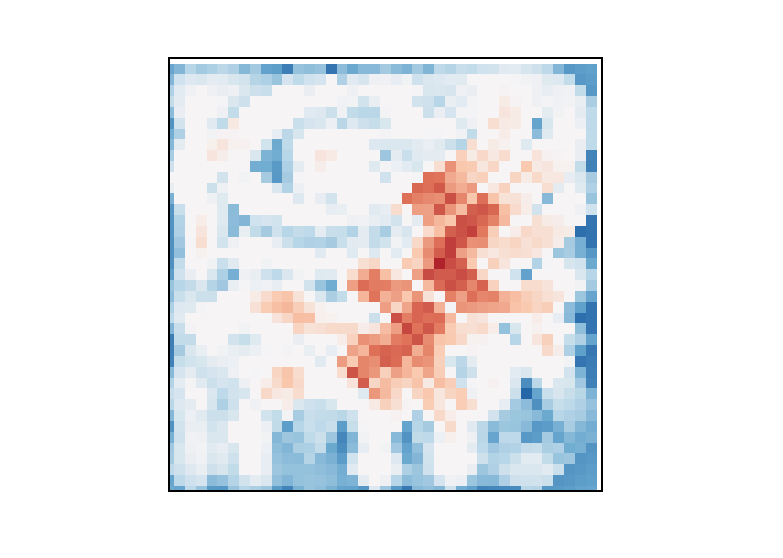
\includegraphics[trim={2.6cm .9cm 2.89cm .8cm},clip, width=\linewidth]{figs/conf/conf_150}}
    \caption{$t = t_0 + 50$}
    \label{subfig:command_heat:conf_150}
  \end{subfigure}
  %\hspace*{1em}
  \begin{subfigure}{.15\linewidth}
    \centering
    \frame{\includegraphics[trim={2.6cm .9cm 2.89cm .8cm},clip, width=\linewidth]{figs/conf/conf_200}}
    \caption{$t = t_0 + 100$}
    \label{subfig:command_heat:conf_200}
  \end{subfigure}
  %\hspace*{.1em} 
  \begin{subfigure}{.0265\linewidth}
    \includegraphics[width=\linewidth]{{figs/cbar/cbar_confidence}}      
  \vspace*{.25em}     
  \end{subfigure}
\\  
\begin{subfigure}{0.3\linewidth}
    \centering
        \includegraphics[height=.8\linewidth]{{figs/temp_attraction_confidence}}
        \caption{Attraction}
        \label{subfig:command_range:attract}
    \end{subfigure}
    \hspace*{2em}
    \begin{subfigure}{0.3\linewidth}
    \centering
        \includegraphics[trim={2.6cm 0cm 0cm 0cm},clip, height=.8\linewidth]{{figs/temp_repulsion_confidence}}
        \caption{Repulsion}
        \label{subfig:command_range:repluse}
    \end{subfigure}      
  \caption
    {An example of the operator's command at $t_0$ (a), the agent's confidence map before (b) and after receiving the command (c), and after moving to the center (d and e). (f) and (g) show the influence of the operator's command at $t=300$ on the swarm's confidence. \label{fig:command_heat}}
\end{figure}

\subsection{\textcolor{red}{Human interaction}}
In another set of experiments, we observe the behavior of the swarm with the operator's intervention. %Fig.~\ref{fig:command_heat} shows the swarm before the operator commands the agents to explore a region in middle of the mission zone. 
The operator can lead the swarm to explore an area of interest (attraction) or prevent them from flying over a no-fly zone (repulsion) by manipulating its own confidence map and disseminating it to a neighboring agent (i.e., O(1)). For example, the operator can send a new confidence map with attraction in the middle to its neighboring agent (see Fig.~\ref{subfig:command_heat:command}). As the agents continuously update their confidence map based on their neighbors, they notice the imposed change in the confidence map and some of them move towards the middle area to compensate the confidence (see Fig.~\ref{subfig:command_heat:conf_200}). %As a result, they follow the operator's command.
Fig.~\ref{fig:command_heat} shows the influence of the operator's command on the confidence of a random agent and how the agent is controlled. Fig.~\ref{subfig:command_heat:command} illustrates the confidence map that the operator introduces to the swarm to attract them to the middle of the arena. After receiving the command, the agent computes the mean of its previous confidence map (see Fig.~\ref{subfig:command_heat:conf_100}) and the command to update its map (see Fig.~\ref{subfig:command_heat:conf_101}). As a result of the attraction force, the agents move towards the area in the middle and this influence diminishes. The agents' presence in the middle of the arena can be seen as the confidence values increase in the middle (see Figs.~\ref{subfig:command_heat:conf_150} and~\ref{subfig:command_heat:conf_200}). 
% \begin{figure}
%     \centering
% \begin{subfigure}{0.3\linewidth}
%     \centering
%         \includegraphics[height=.8\linewidth]{{figs/temp_attraction_confidence}}
%         \caption{Attraction}
%         \label{subfig:command_range:attract}
%     \end{subfigure}
%     \hspace*{2em}
%     \begin{subfigure}{0.3\linewidth}
%     \centering
%         \includegraphics[trim={2.6cm 0cm 0cm 0cm},clip, height=.8\linewidth]{{figs/temp_repulsion_confidence}}
%         \caption{Repulsion}
%         \label{subfig:command_range:repluse}
%     \end{subfigure}    
%     \caption{{The influence of the operator's command on the swarm's confidence. Results from the median values from $15$ runs show the effect of the operator's command on the confidence of the swarm. The commands are issued at $t=300$.}}
%     \label{fig:command_range}
% \end{figure}
%\textcolor{red}{attraction effect on confidence map with different communication range... }
%\textcolor{red}{repulsion effect on confidence map with different communication range...}
The operator's command message reaches the agents that are in its local neighborhood and the communication range determines the impact on the swarm. %Fig.~\ref{fig:command_range} shows {how different communication ranges between human-swarm affects the confidence level of the agents}. We examined the behavior of the swarm with three communication ranges, $r = \{50, 100, 150\}$ (arena size is $600 \times 600$ pixels). 
With wider communication ranges, the operator influences more agents and therefore the effect is more significant. In case of attraction, agents quickly move to the cell with low confidence and immediately compensate the drop in the certainty level, while in repulsion the agents cannot visit the cell to recover from the added value to the confidence as they are repelled from that region. This explains the recovery of the confidence levels in Fig.~\ref{subfig:command_range:attract} and the bias that stays in the swarm for the rest of the experiment in Fig.~\ref{subfig:command_range:repluse}. At $t=300$ the operator disseminates the commands once and it takes 100 to 200 simulation steps to significantly influence the swarm.
\begin{figure}
    \centering
    % \hspace{0.6\textwidth} 
    %  \begin{subfigure}[b]{.3\textwidth}
    %     \centering
    %     {\includegraphics[width=\textwidth]{figs/lines/repulsion}}     
    %     %\vspace*{2em} 
    % \end{subfigure}     
    % \\
    \begin{subfigure}[b]{0.15\textwidth} %-------------------------------------
    \centering
        \includegraphics[trim={2.5cm .8cm 3cm .7cm},clip, height=\linewidth]{{figs/cmd/constant_repulsion_command}}        %\caption{belief error with repulsion\textcolor{red}{, several communication range}}
        %\vspace{0.44em}
        \caption{Command}
        \label{subfig:permanent_command:command}
    \end{subfigure} 
    %\hspace{.00035\textwidth}    
     \begin{subfigure}[b]{.0255\textwidth} %confidence legend
        \centering
        {\includegraphics[width=\textwidth]{figs/cbar/cbar_confidence.pdf}}     
        %\vspace*{-1.62em} 
        \vspace{0.45em}
    \end{subfigure}     
    %\centering    
    %          influence ende
    %%
    %         coverage begin
    %\hspace{0.0004\textwidth}
    %\hspace*{2em}
    \begin{subfigure}[b]{0.15\textwidth}%---------------------------------------
    \centering
        \includegraphics[trim={0cm 0cm 0cm 0cm},clip, height=\linewidth]{{figs/cmd/distribution_constant_repulsion}}        %\caption{belief error with repulsion\textcolor{red}{, several communication range}}
        %\vspace{0.44em}
        \caption{Coverage}
        \label{subfig:permanent_command:distribution}
        
    \end{subfigure} %% end of coverage heatmap
     \begin{subfigure}[b]{.03\textwidth} % coverage legend begins
        \centering
        
        {\includegraphics[width=\textwidth]{figs/cbar/cbar_distribution.pdf}}     
        \vspace{0.4em}
    \end{subfigure}      
%        \caption{A repulsion command that is sent throughout the runtime by the operator to the agents in range (a) and the average distribution of agents in all simulation runs (b). The experiment shows that agents hardly cross the area in the middle and move around the arena for exploration.} 
%        \label{fig:dist_permanent_repulsion}
%\end{figure}    
%\begin{figure}
%    \centering
%    \hspace{1em}
    % \hspace{0.02\textwidth}
    % \begin{subfigure}[b]{0.27\textwidth}%------------------------
    % \centering
    %     %\captionsetup{justification=centering, margin =2.6cm}    
    %     \includegraphics[height=.8\textwidth]{{figs/belief_permanent_repulsion}}
    %     %\vspace*{-1em} 
    %     %vspace{0.0001em}
    %     \caption{Belief error}
    %     \label{subfig:permanent_command:belief_error}
    % \end{subfigure}    
    % \hspace{0.02\textwidth}
    % \begin{subfigure}[b]{0.27\textwidth}
    % \centering
    %     \includegraphics[height=.8\textwidth]{{figs/conf_permanent_repulsion}}
    %     %\vspace*{-1em} 
    %     \caption{Confidence}
    %     \label{subfig:permanent_command:confidence}
    % \end{subfigure}    
    \begin{subfigure}[b]{0.15\linewidth}
    \centering
        %\captionsetup{justification=centering, margin =2.6cm}    
        \frame{\includegraphics[trim={.2cm .05cm .2cm .7cm},clip,height=\linewidth]{{figs/scr/maz_100}}}
        \caption{$L$}
        \label{subfig:operator_barriers:maze_100}
    \end{subfigure}    
    % \begin{subfigure}{0.15\linewidth}
    % \centering
    %     \frame{\includegraphics[trim={.2cm .05cm .2cm .7cm},clip,height=.8\linewidth]{{figs/scr/maz_120}}}
    %     \caption{$1.2L$}
    %     \label{subfig:belief_conf_permanent_repulsion_range:conf_repulse}
    % \end{subfigure}    
    % \begin{subfigure}{0.15\linewidth}
    % \centering
    %     %\captionsetup{justification=centering, margin =2.6cm}    
    %     \frame{\includegraphics[trim={.2cm .05cm .2cm .7cm},clip,height=.8\linewidth]{{figs/scr/maz_140}}}
    %     \caption{$1.4L$}
    %     \label{subfig:belief_conf_permanent_repulsion_range:belief_repluse}
    % \end{subfigure}    
    % \begin{subfigure}{0.15\linewidth}
    % \centering
    %     %\captionsetup{justification=centering, margin =2.6cm}    
    %     \frame{\includegraphics[trim={.2cm .05cm .2cm .7cm},clip,height=.8\linewidth]{{figs/scr/maz_160}}}
    %     \caption{$1.6L$}
    %     \label{subfig:belief_conf_permanent_repulsion_range:belief_repluse}
    % \end{subfigure}    
    \begin{subfigure}[b]{0.15\linewidth}
    \centering
        %\captionsetup{justification=centering, margin =2.6cm}    
        \frame{\includegraphics[trim={.2cm .05cm .2cm .7cm},clip,height=\linewidth]{{figs/scr/maz_180}}}
        %\vspace{2.0em}
        \caption{$1.8L$}
        \label{subfig:operator_barriers:maze_180}
    \end{subfigure}    
%     \caption{Different complexity level of a barrier}
%     \label{fig:belief_conf_permanent_repulsion_range}
% % \end{figure}
% % \begin{figure}% >>>
% %     \centering
% % %        \begin{subfigure}{0.4\linewidth}
% %             \includegraphics[width=.4\linewidth]{{figs/operator_belief_error_all_barriers}}
% %         \caption
% %         {A map of a mission zone with agents, a disaster, and a human operator. All agents and the operator have belief and confidence maps with a lower resolution compared to the actual images.\label{fig:scr_map}}
% % \end{figure}
% \begin{figure}
    %\centering
    \begin{subfigure}{.3\linewidth}
    \centering
        %\captionsetup{justification=centering, margin =2.6cm}    
        \includegraphics[height=.8\linewidth]{{figs/operator_belief_error_all_barriers}}
        \caption{Effect of barrier size}
        \label{subfig:operator_barriers:belief_error}
    \end{subfigure}    
    \hspace*{.1em}
    \begin{subfigure}{.09\textwidth}
        \centering
        {\includegraphics[width=\textwidth]{figs/lines/maze_line}}     
        \vspace*{2em} 
    \end{subfigure}      
    \caption{Operator's confidence map for introducing a permanent repulsion (a) and the swarm's distribution (b). Error in the operator's belief map for different sizes of the repulsion zones. The precision of the belief map decreases as the size of the barrier grows. For the barrier of length 1.8L the operator will no longer be able to receive precise mapping of the environment (e).
    % and the median error in belief map (c) and the confidence level of the swarm (d) with (blue) and without permanent repulsion force (red).
    }
    \label{fig:permanent_command}
\end{figure}
    In another experiment, we assumed a disaster situation where agents must avoid a certain area at all time. An example would be the frequent flying zone of an airport or a no-fly area with high voltage cables. For that, the operator can continuously apply a repulsion force in the prohibited zone.
Fig.~\ref{subfig:permanent_command:command} shows the confidence bias that the operator introduces to the swarm. The cells highlighted with red mark the prohibited zone. The blue area can be either empty which allows the swarm to keep the knowledge about the confidence and only manipulate the values in the interest zone or {can be set to zero that would gradually decrease the agents' confidence level.} Fig.~\ref{subfig:permanent_command:distribution} shows the distribution of the agents in all simulation runs with the permanent repulsion at the center. It is clear in this figure that the operator successfully controlled the swarm to avoid the area in the middle of the mission zone. As the communication range is limited, it takes a short time until all agents become aware of the new force introduced by the operator. Therefore, a few pixels in the prohibited zone show that some agents crossed this area. The ring in the distribution around the prohibited zone is caused by the area with the equilibrium between different repulsion forces.  
%\textcolor{red}{permanent repulsion effect on belief \& confidence map ... }
%constant_repulsion_command
%Fig.~\ref{fig:belief_conf_permanent_repulsion_range} shows that the swarm is able to map the environment with a prohibited zone with a minor increase in the error level compared to the experiment without any limits (a wider space is available for the swarm motion). The difference in the confidence level is only due to the added confidence value by the operator to all agents. 
% \begin{figure}
%     \centering
%     %\hspace{1em}
%     \begin{subfigure}{0.15\linewidth}
%     \centering
%         %\captionsetup{justification=centering, margin =2.6cm}    
%         \frame{\includegraphics[trim={.2cm .05cm .2cm .7cm},clip,height=.8\linewidth]{{figs/scr/maz_100}}}
%         \caption{$L$}
%         \label{subfig:operator_barriers:maze_100}
%     \end{subfigure}    
%     % \begin{subfigure}{0.15\linewidth}
%     % \centering
%     %     \frame{\includegraphics[trim={.2cm .05cm .2cm .7cm},clip,height=.8\linewidth]{{figs/scr/maz_120}}}
%     %     \caption{$1.2L$}
%     %     \label{subfig:belief_conf_permanent_repulsion_range:conf_repulse}
%     % \end{subfigure}    
%     % \begin{subfigure}{0.15\linewidth}
%     % \centering
%     %     %\captionsetup{justification=centering, margin =2.6cm}    
%     %     \frame{\includegraphics[trim={.2cm .05cm .2cm .7cm},clip,height=.8\linewidth]{{figs/scr/maz_140}}}
%     %     \caption{$1.4L$}
%     %     \label{subfig:belief_conf_permanent_repulsion_range:belief_repluse}
%     % \end{subfigure}    
%     % \begin{subfigure}{0.15\linewidth}
%     % \centering
%     %     %\captionsetup{justification=centering, margin =2.6cm}    
%     %     \frame{\includegraphics[trim={.2cm .05cm .2cm .7cm},clip,height=.8\linewidth]{{figs/scr/maz_160}}}
%     %     \caption{$1.6L$}
%     %     \label{subfig:belief_conf_permanent_repulsion_range:belief_repluse}
%     % \end{subfigure}    
%     \begin{subfigure}{0.15\linewidth}
%     \centering
%         %\captionsetup{justification=centering, margin =2.6cm}    
%         \frame{\includegraphics[trim={.2cm .05cm .2cm .7cm},clip,height=.8\linewidth]{{figs/scr/maz_180}}}
%         \caption{$1.8L$}
%         \label{subfig:operator_barriers:maze_180}
%     \end{subfigure}    
% %     \caption{Different complexity level of a barrier}
% %     \label{fig:belief_conf_permanent_repulsion_range}
% % % \end{figure}
% % % \begin{figure}% >>>
% % %     \centering
% % % %        \begin{subfigure}{0.4\linewidth}
% % %             \includegraphics[width=.4\linewidth]{{figs/operator_belief_error_all_barriers}}
% % %         \caption
% % %         {A map of a mission zone with agents, a disaster, and a human operator. All agents and the operator have belief and confidence maps with a lower resolution compared to the actual images.\label{fig:scr_map}}
% % % \end{figure}
% % \begin{figure}
%     \centering
%     \begin{subfigure}{.3\textwidth}
%     \centering
%         %\captionsetup{justification=centering, margin =2.6cm}    
%         \includegraphics[height=.8\linewidth]{{figs/operator_belief_error_all_barriers}}
%         \caption{test}
%         \label{subfig:operator_barriers:belief_error}
%     \end{subfigure}    
%     \hspace*{.1em}
%     \begin{subfigure}{.09\textwidth}
%         \centering
%         {\includegraphics[width=\textwidth]{figs/lines/maze_line}}     
%         \vspace*{2em} 
%     \end{subfigure}     
%     \caption{{Error in the operator's belief map for different sizes of the repulsion zones. The precision of the belief map decreases as the size of the barrier grows. For the barrier of length 1.8L the operator will no longer be able to receive precise mapping of the environment.}}
%     \label{fig:operator_barriers}
% \end{figure}
In another experiment, we simulated the influence of five permanent no-fly zones with a bar of length L to 1.8L (see Figs.~\ref{subfig:operator_barriers:maze_100}-\ref{subfig:operator_barriers:maze_180}). Fig.~\ref{subfig:operator_barriers:belief_error} shows the error in the operator's belief map with different sizes of the repulsion zones and without any barriers. As the barrier grows in size, the precision of the mapping decreases. For 1.8L the barrier is too spacious for the swarm to keep the operator updated about the situation and the precision of the belief map decreases significantly (i.e., the belief error does not decline over time). The operator can disseminate arbitrary maps of repulsion or attractions. Our results show that the swarm is able to follow the control commands and continue to offer a precise mapping of the environment.

\begin{figure}
    \centering
    %\hspace*{3em}
    \begin{subfigure}{.15\linewidth}
    \centering
        \includegraphics[width=\linewidth]{{figs/change/change}}
        \caption{$t = (t_0,t_1)$}
        \label{subfig:change:change_scr}
    \end{subfigure}   
    \hspace*{.15em}
    % \begin{subfigure}{.15\linewidth}
    % \centering
    %     \includegraphics[trim={2.5cm 1.5cm 3.6cm .78cm},clip, width=\linewidth]{{figs/change/belief_299}}
    %     \caption{$t = t_0$}
    %     \label{subfig:change:belief_300}
    % \end{subfigure}
    % % \hspace*{.15em}
    \begin{subfigure}{.15\linewidth}
    \centering
        \includegraphics[trim={2.5cm 1.5cm 3.6cm .78cm},clip, width=\linewidth]{{figs/change/belief_350}}
        \caption{$t = t_1$}
        \label{subfig:change:belief_350}
    \end{subfigure}    
     \hspace*{.15em}
    \begin{subfigure}{.15\linewidth}
    \centering
        \includegraphics[trim={2.5cm 1.5cm 3.6cm .78cm},clip, width=\linewidth]{{figs/change/belief_550}}
        \caption{$t = t_1 + 200$}
        \label{subfig:change:belief_550}
    \end{subfigure}    
    \hspace*{.15em}
    \begin{subfigure}{.15\linewidth}
    \centering
        \includegraphics[trim={2.5cm 1.5cm 3.6cm .78cm},clip, width=\linewidth]{{figs/change/belief_750}}
        \caption{$t = t_1 + 400$}
        \label{subfig:change:belief_750}
    \end{subfigure}
    \hspace*{.15em}
    \begin{subfigure}{.15\linewidth}
    \centering
        \includegraphics[trim={2.5cm 1.5cm 3.6cm .78cm},clip, width=\linewidth]{{figs/change/belief_950}}
        \caption{$t = t_1 + 600$}
        \label{subfig:change:belief_950}
    \end{subfigure}
    % \hspace*{.05em}
     \begin{subfigure}{.03\linewidth}
        \centering
        {\includegraphics[width=\linewidth]{figs/cbar/cbar_belief.pdf}}     
        \vspace*{.3em}                
    \end{subfigure}       
    %\hspace*{4em}   
    \\
    \begin{subfigure}{.3\linewidth}
    \centering
        \includegraphics[height=.8\linewidth]{{figs/change/belief_change}}
        \caption{Swarm's belief error}
        \label{subfig:change:swarm_belief_error}
    \end{subfigure}
    \hspace*{2em}
     \begin{subfigure}{.3\linewidth}
        \centering
        \includegraphics[height=.8\linewidth, trim={2.4cm 0cm 0cm 0cm}, clip,]{{figs/change/operator_belief_change}}
        \caption{Operator's belief error}
        \label{subfig:change:op_belief_error}
    \end{subfigure} 
        
    \caption{The disaster zone moves between $t_0$ and $t_1$ (green area in (f and g)). The agent gradually adapts itself to the change (b-e). Median error in belief maps of the swarm (f) and {the operator (g)} when the disaster zone moves. %During a slow displacement phase $[t_0=150 < t < t_1=350]$, highlighted with the green bar, a major increase in the error is observed. The swarm recovers and the error in the swarm's and the operator's belief map declines.
    }
    \label{fig:change}
\end{figure}

\subsection{\textcolor{red}{Response to evolving disaster}}
We also examined the robustness of our approach in a dynamic environment with an evolving disaster. We assume that the disaster zone is not fixed and it can move to another point in the area and observe how this change is reflected in the performance of the swarm and the operator's understanding of the environment. Fig.~\ref{fig:change} shows that in case of changes in the environment the operator stays updated. Fig.~\ref{subfig:change:change_scr} shows the direction of the disaster displacement. Fig.~\ref{subfig:change:belief_350} shows the belief map when the motion is stopped. 
%We can see that the belief map already reflects the change and the operator learns about the trace of the disaster as a potential disaster zone. 
Gradually the operator's belief map adapts to the new position of the disaster (see Figs.~\ref{subfig:change:belief_350}-\ref{subfig:change:belief_950}). Fig.~\ref{fig:change:boxplot} shows the effect of a dynamic environment on the error in the belief of the swarm (see Fig.~\ref{subfig:change:swarm_belief_error}) and the operator (see Fig.~\ref{subfig:change:op_belief_error}) over time. The disaster zone moved between $150 < t < 350$ simulation steps. %A correct belief map of the environment consists of 14 cells with the value one and other cells set to zero. 
The swarm continuously adapts to the change by decreasing the belief in the former position of the disaster and starting to increase the belief in the new positions. This behavior can be seen in Figs.~\ref{subfig:change:belief_350}-\ref{subfig:change:belief_950} by the former positions of the disaster slowly fading away and the new positions appearing in the belief maps. This process continues until the environment becomes stable and the error declines again. Shortly after, the agents successfully map the environment and notify the operator. The results from the evolving disaster experiment shows that the swarm is resilient to changes in the environment and the operator's belief map stays updated. 

%\textcolor{red}{conclude the results}

% \begin{figure}
    
%     %\hspace*{4em}   
%     \centering
%     \begin{subfigure}{.3\linewidth}
%     \centering
%         \includegraphics[height=.8\linewidth]{{figs/change/belief_change}}
%         \caption{Swarm's belief error}
%         \label{subfig:change:belief_error}
%     \end{subfigure}
%     \hspace*{2em}
%      \begin{subfigure}{.3\linewidth}
%         \centering
%         \includegraphics[height=.8\linewidth, trim={2.4cm 0cm 0cm 0cm}, clip,]{{figs/change/operator_belief_change}}
%         \caption{Operator's belief error}
%         \label{subfig:change:op_belief}
%     \end{subfigure} 
    
%     \caption{Median error in belief maps of the swarm (a) and \textcolor{blue}{the operator (b)} when the disaster zone moves. During a slow displacement phase ($150 < t < 350$), highlighted with the green bar, a major increase in the error is observed. The swarm recovers and the error declines after the disaster is fixed.}
%     \label{fig:change:boxplot}
% \end{figure}
\section{Conclusion and Future Work}
\label{sec:conclusion}
We proposed and implemented a scalable and adaptive human-swarm interaction method and evaluated the performance of a simulated swarm of agents in disaster management. We showed that a human operator does not require a fully connected communication channel with all agents to be able to monitor the swarm and control them. In our experiments, an operator controlled $15$ simulated agents that successfully explored the environment even when its dynamic. There are several directions that this research can be extended and further developed. We plan to investigate the effect of multiple dynamic disaster areas and human operators with collaborative/competitive disaster management strategies. Besides the contradictory operator commands, there may also be intruder attacks by other agents or operators that need to be detected and eliminated from the decision-making process. %Another direction to build on this research is to predict the evolution of the disaster zone over time.
%Finding the optimum swarm size and operator groups in a human-swarm teams is also a potential research direction. 
We plan to address some of these challenges and implement our approach on physical unmanned aerial vehicles and evaluate the performance of the swarm in real world applications. 
%more information from the swarm including detecting faulty robots in the swarm

%\newpage

%
% ---- Bibliography ----
%
%\bibliographystyle{dars/styles/bibtex/splncs03}
\bibliographystyle{splncs04}
\bibliography{bib}
\end{document}
